\subsection{Prototype-update decisions: fixed protocol and evidence cutoff}\label{sec:paired-experiments}
The new campaign addresses a specific decision: does a proposed prototype
update strictly reduce the exact quantized nearest-center cost on the unchanged
private audit catalog? This is distinct from predicting labels or proving that
a particular model-training algorithm was followed. The snapshot in this
revision was captured on 22 October 2026 at 12:32 UTC. It includes all completed
native results and 15 of 32 main proof cases, plus a separate completed
portability case. The captured tables below retain that frozen evidence boundary. On 23 October,
the server console reported completion of both the main and scale queues.
Appendix~\ref{sec:scale-console} separately reports provisional scale results;
uncaptured main cases are not added to the verified tables or success counts.

The predeclared numerical grid uses MNIST, Fashion-MNIST and 2,000-feature
20 Newsgroups TF--IDF, $k=3,5,10$, and seeds 11/23/37/41/53. Each source is capped
at 5,000 rows before zero-norm removal. A seeded 60/40 split supplies training
and held-out audit rows; the first 1,024 audit rows form the native catalog,
and its first 128 rows form proof inputs. The input scale is
$4095/\max|\text{training}|$, with audit coordinates clipped to the approved
range and clipping recorded. The TF--IDF source vocabulary is constructed
before this split: these are held-out rows of a fixed feature catalog, not a
claim of an inductive text-preprocessing pipeline.

Training-only Lloyd traces run for 24 steps after seeded $k$-means++
initialization. Early baselines at step 1 are compared with steps 2/4/8/16;
mature baselines at step 8 with steps 9/12/16/24. Each task also retains a null
and reverse-step diagnostic. No update uses audit outcomes to fit its centers.
Head and PCA bases use training rows only: a rank-63 centroid-informed/residual
PCA basis or ordinary PCA, with nested rank-15 prefixes and common $T=16384$.
The historical scale/precision configuration in Section~\ref{sec:review-controls}
is a separate cohort.

There are 45 fitted prototype configurations across 15 dataset/split-seed
replications, two dependent baseline ages, two methods and two ranks:
2,160 numerical cells, including 1,440 actual update requests. Different $k$,
ages, ranks and updates share each dataset/seed split and are not independent
statistical observations. All cells, unchanged controls, PCA wins and
inconclusive outcomes are retained. Every absolute and paired interval contains
the exact integer reference, and no certified assignment is incorrect in these
checks. Finite checks support implementation consistency; the propositions
supply the deterministic bounds.

\subsection{Native decision usefulness and representation comparison}
Table~\ref{tab:paired-native} separates three quantities: the frequency of a
conclusive cost-change sign, guaranteed assignment coverage, and observed
assignment agreement. At rank 63, early-update sign decisions resolve 100\% of
MNIST requests and 80\% of Fashion-MNIST requests for both representations,
but none of the text requests. Mature updates are mostly inconclusive:
MNIST rates are 18.33\% for head and 13.33\% for PCA, Fashion-MNIST 10\% for both,
and text zero for both. A small cost change can be difficult to certify even
when most assignments have a certificate.
\begin{table*}[tp]
\centering
\small
\caption{Independent-fit numerical grid at rank 63: update decisions, assignment coverage and agreement (percent).}\label{tab:paired-native}
\begin{tabular}{lrrrrrrr}
\toprule
Dataset & Age & Decision L & Decision P & Coverage L & Coverage P & Agreement L & Agreement P \\
\midrule
MNIST & Early & 100.00 & 100.00 & 92.65 & 87.91 & 99.74 & 99.82 \\
MNIST & Mature & 18.33 & 13.33 & 96.57 & 91.52 & 99.92 & 99.79 \\
Fashion-MNIST & Early & 80.00 & 80.00 & 97.51 & 94.99 & 99.94 & 99.93 \\
Fashion-MNIST & Mature & 10.00 & 10.00 & 98.93 & 96.93 & 99.98 & 99.95 \\
20NG TF--IDF & Early & 0.00 & 0.00 & 0.32 & 0.13 & 93.66 & 93.54 \\
20NG TF--IDF & Mature & 0.00 & 0.00 & 10.16 & 0.80 & 97.78 & 95.71 \\
\bottomrule
\end{tabular}
\par\smallskip\begin{minipage}{0.98\linewidth}\footnotesize L: centroid-informed head plus residual PCA; P: PCA plus energy. Each row summarizes 60 dependent update requests from 15 fitted $k$/seed configurations. Both methods use the same held-out rows, updates, rank and precision. Decision rate is the fraction with a certified strict cost-change sign; assignment agreement is against quantized Full. These are numerical results, not proof timings.\end{minipage}
\end{table*}


Across early rank-63 requests, independently subtracted absolute intervals
resolve 57.78\% for head and 25.00\% for PCA; paired bounds resolve 60.00\% for
both. The early fit-level paired-decision comparison is 45 ties and no wins or
losses for head against PCA. For mature fits it is two head wins and 43 ties.
These outcomes support a representation-agnostic audit interface rather than
uniform learned superiority. At rank 15, early head resolves no actual update
requests and PCA resolves 6.67\%; mature rates are zero and 2.78\%.

The original $N=1024$ headline workload remains a negative decision example:
all nine updated absolute cost intervals overlap each other and the baseline
interval. No strict ordering follows from interval separation. Its 98.25\%
observed agreement and 5.08-fold component-cost ratio do not establish useful
update decisions by themselves. The new Lloyd-trace tasks test a different,
explicitly reported workload rather than repairing that original result.

\subsection{Natural regressions and the audit decision boundary}
A sign-stratified reanalysis counts the 360 actual rank-63 requests once per
fitted task, rather than once per representation. Of these, 336 improve the
held-out cost and 24 worsen it: ten MNIST and fourteen Fashion-MNIST requests.
All 24 regressions occur in mature-update tasks. Both head and PCA return
inconclusive on every one; neither directly certifies a natural worsening.
Table~\ref{tab:natural-regressions} exposes the breakdown without counting the
reverse diagnostic as a natural regression.
\begin{table*}[t]
\centering\small
\caption{Rank-63 native decisions stratified by the true held-out cost change. Only actual Lloyd updates are counted; null and reverse diagnostics are excluded. Each request is evaluated by both methods.}\label{tab:natural-regressions}
\begin{tabular}{llrrrr}
\toprule
Dataset & Age & Improving & Resolved H/P & Worsening & Resolved H/P \\
\midrule
MNIST & Early & 60 & 60/60 & 0 & 0/0 \\
MNIST & Mature & 50 & 11/8 & 10 & 0/0 \\
Fashion-MNIST & Early & 60 & 48/48 & 0 & 0/0 \\
Fashion-MNIST & Mature & 46 & 6/6 & 14 & 0/0 \\
20NG TF--IDF & Early & 60 & 0/0 & 0 & 0/0 \\
20NG TF--IDF & Mature & 60 & 0/0 & 0 & 0/0 \\
\bottomrule\end{tabular}
\end{table*}


This is a limitation of the uncertainty envelope, not an incorrect approval:
a policy that approves only a certified decrease would defer all 24 tasks to
exact fallback. It does not follow that inconclusive tasks are regressions;
many genuine improvements are also inconclusive. The reverse-step example
checks worsening semantics but does not establish practical regression
sensitivity. The evidence supports selective improvement certification on
early image traces, not a demonstrated low-cost detector of harmful deployed
updates. Mature traces are the more relevant negative test for that motivation.

\subsection{Completed proof costs and a matched deployment}\label{sec:paired-proof-results}
Six fitted proof workloads were fixed before inspecting the numerical grid:
MNIST/$k=3$/seed 11, Fashion-MNIST/$k=5$/seed 11, text/$k=10$/seed 11,
MNIST/$k=10$/seed 23, Fashion-MNIST/$k=3$/seed 23 and text/$k=5$/seed 23.
Each requests head/PCA at ranks 15/63 and exact reusable Full. Two additional
one-repetition deployment controls give 32 planned cases. Within each fit,
precision, rows, centers, query batch and timing repetitions match. Stage~1
binds every row once. The first MNIST fit uses three timed query repetitions
and one warmup; other fits use one timed repetition without warmup. Image
batches contain four rows; text/$k=10$ uses one and text/$k=5$ two under the
1.6-million-constraint guard. Proof counts measure execution coverage, not
independent learning problems.

All first-fit MNIST and Fashion alternatives and text rank-63/Full alternatives
have completed at the cutoff. Each completed worker separately replays the
chosen relation using public-only exports and independently approved pins/tasks.
Table~\ref{tab:paired-costs} reports each completed alternative, including
inconclusive ones. It charges native preparation, shared row binding, query
compilation/setup, native answer construction, witness/proving, paired
public-parameter preparation and phase-specific public replay. Exploratory
absolute-certificate proofs are not charged to the paired alternative.
\begin{table*}[tp]
\centering
\small
\caption{Completed N=128 proof alternatives at the snapshot cutoff. Cost includes phase-specific public replay.}\label{tab:paired-costs}
\begin{tabular}{lrrrrrr}
\toprule
Workload & $k$ & Method & Rank & Batch & Cost (min) & Decisions \\
\midrule
MNIST & 3 & Full & -- & 4 & 33.81 & 4/4 \\
MNIST & 3 & Head & 63 & 4 & 17.04 & 4/4 \\
MNIST & 3 & Head & 15 & 4 & 10.38 & 0/4 \\
MNIST & 3 & PCA & 63 & 4 & 16.74 & 4/4 \\
MNIST & 3 & PCA & 15 & 4 & 10.44 & 0/4 \\
Fashion-MNIST & 5 & Full & -- & 4 & 34.62 & 4/4 \\
Fashion-MNIST & 5 & Head & 63 & 4 & 17.28 & 4/4 \\
Fashion-MNIST & 5 & Head & 15 & 4 & 12.27 & 0/4 \\
Fashion-MNIST & 5 & PCA & 63 & 4 & 17.48 & 4/4 \\
Fashion-MNIST & 5 & PCA & 15 & 4 & 12.34 & 0/4 \\
20NG TF--IDF & 10 & Full & -- & 1 & 118.40 & 4/4 \\
20NG TF--IDF & 10 & Head & 63 & 1 & 108.60 & 0/4 \\
20NG TF--IDF & 10 & PCA & 63 & 1 & 106.33 & 0/4 \\
\bottomrule
\end{tabular}
\par\smallskip\begin{minipage}{0.98\linewidth}\footnotesize Six sets comprise one null control, four actual Lloyd updates and one reverse-step diagnostic; all six are charged, but the last column counts only the four actual updates. Shared row binding is charged once to each reuse alternative. Query medians use three repetitions on the first MNIST fit and one elsewhere; Stage 1 uses one timing per row. All use $T=16384$ and matched batches within each fit. Reconstructed costs exclude fitting, benchmark warmups and process/I/O overhead; they include verifier replay and paired public-parameter preparation. A cheaper inconclusive service is not equivalent to exact Full.\end{minipage}
\end{table*}


The standalone MNIST deployment controls use the same $N=128$, $k=3$, rank 63,
six sets, batch 4 and original root, with one repetition and no warmup.
Measured workflow wall time is 1,054.55\,s for paired reuse and 2,181.77\,s
for exact Full, a 2.07-fold ratio. This includes public replay and process
overhead, excludes prior fitting and subsequent private reference validation,
and resolves all four actual updates without fallback. The null certifies
equality and the reverse-step diagnostic certifies worsening. This is a single
observed deployment, not a timing distribution or a production-throughput claim.
The multi-alternative benchmark wall times are longer because they include
other relations and repeated proofs; they must not replace the selected
alternative costs in Table~\ref{tab:paired-costs}.

\begin{figure*}[tp]
\centering
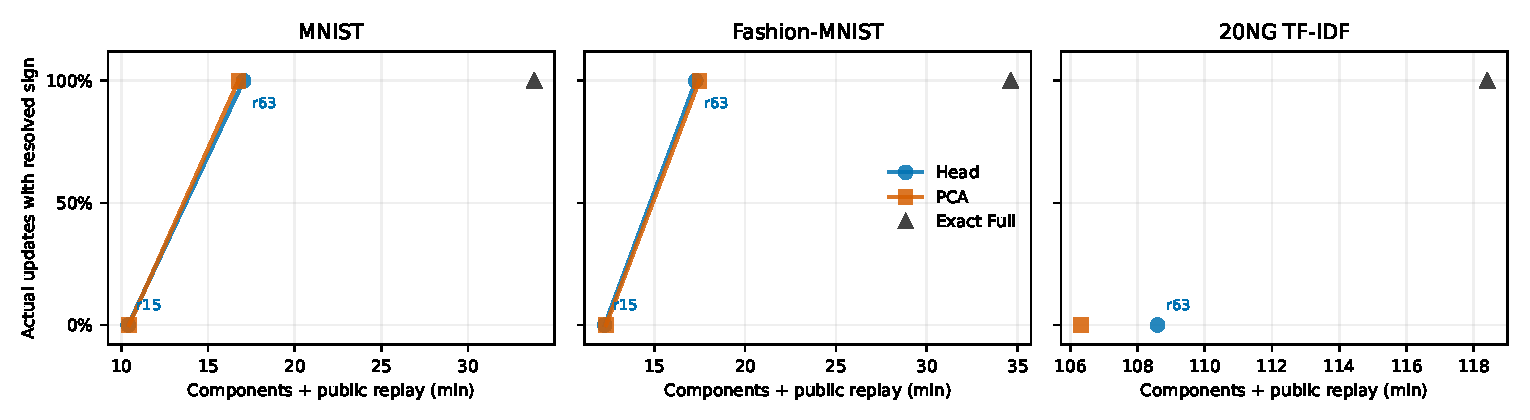
\includegraphics[width=\textwidth]{paper_results/review_controls/paired_20261022/cost_decisions.pdf}
\caption{Completed cost--decision alternatives on three fitted $N=128$ workloads.
Costs are reconstructed publisher components plus measured public replay;
decision rates count four actual updates per fit. Image points span nested
ranks 15/63 at fixed precision and batching. Text rank 15 points were not captured at the table cutoff.
Head/PCA rank 63 image decision rates coincide. The figure is descriptive:
dependent requests provide no independent confidence interval, and an
inconclusive low-cost point does not provide the same service as Full.}
\label{fig:paired-frontier}
\end{figure*}

Rank-63 paired text costs are 108.60\,min for head and 106.33\,min for PCA,
versus 118.40\,min for Full on the selected component-plus-replay boundary.
Both approximate alternatives resolve zero of four updates. Thus their modest
cost reduction does not establish a useful acceleration; adding exact fallback
can cost more than using Full directly. Rank15 image proofs are cheaper but
also resolve none of the actual updates on these fitted proof examples.

The larger paired scale queue reported completion through the server console.
Its provisional timings and locally checked input quality are isolated in
Appendix~\ref{sec:scale-console}, outside the captured proof frontier.

\subsection{Fallback, residual diagnosis and resource evidence}
Fresh local public-only audits pass for the captured MNIST and Fashion rank 63
examples. A separate MNIST rank 15 audit is inconclusive on all five non-null
tasks. Selecting and verifying exact Full proofs resolves four improvements
and one worsening; the null is certified equal without fallback. The auditor
reads public exports and approved tasks, not private records or assignment
flags. Its 13.97\,s composed replay time measures verifier-side selection and
verification of saved proofs, not online generation of the fallback proofs.
The implementation demonstrates the decision semantics while leaving a
prospective on-demand fallback service unmeasured.

A numerical diagnostic on the three completed head/rank 63 proof inputs
explains one certificate limitation. Median residual energy relative to
centered original-row energy is 14.49\% for MNIST, 6.95\% for Fashion-MNIST and
89.33\% for text. On the text fit, residual uncertainty supplies 99.79\% of the
assignment-envelope error budget, and the median minimum assignment
gap-to-uncertainty ratio is 0.075; certification requires a ratio above one.
Its assignment coverage over the four updates is zero, although observed
agreement is 91.41\%. These are three individual fitted examples, not a
universal property of image and text modalities. They distinguish a valid
cryptographic proof from a decisive approximation guarantee.

The resource export records serialized proving/verification keys, proof and
public-witness bytes, stored head/energy scalars, public model/task sizes and
fitting times. Table~\ref{tab:paired-resources} reports the first fitted MNIST
alternatives. Network latency, production concurrency and deployment-wide
memory are not measured. The same frozen portability input also completes on
Windows locally and Linux on Mobin with thread caps of four; roots and input
hashes match. One portability example does not provide cross-host timing
statistics.

The staged private reproduction artifact passes 9,142 file-hash checks and
fresh local public-only replay of 7,888 proofs across 20 bundles: fourteen
earlier completed controls, four selected new real-data bundles and two
synthetic relation checks. This is an artifact verification count, not 7,888
independent experiments or a fresh replay of every unfinished campaign case.
Valid-range changes to approved centers or signed endpoints fail verification.
The previous paper's old root/key/task trust assumptions remain necessary.
